\documentclass{report}


%\documentclass{article}    %comento la linea porque ya esta definido
\usepackage[T1]{fontenc}
\usepackage[utf8]{inputenc}
\usepackage{float}
\usepackage{graphicx}
\usepackage{geometry}
\usepackage{titlesec, blindtext, color}
\definecolor{gray75}{gray}{0.75}
\newcommand{\hsp}{\hspace{20pt}}
\titleformat{\chapter}[hang]{\Huge\bfseries}{\thechapter\hsp\textcolor{gray75}{|}\hsp}{0pt}{\Huge\bfseries}

\geometry{
     a4paper,
     left=19mm,
     right=19mm,
     top=19mm,
     bottom=25mm,
     }
     
\usepackage{sectsty}
\allsectionsfont{\normalfont \scshape}


\usepackage{subfiles}						%MULTIARCHIVOS, NO BORRAR
\usepackage{nomencl}					%Para introducir nomenclaturas/definciones
\usepackage{makecell}					%Para emprolijar celdas de tablas
\usepackage{amsmath}
\usepackage{amssymb}					%simbolos matematicos
\usepackage{upgreek}					%puedo usar \uptau que es como \tau pero con mas rulito
\usepackage{steinmetz}
\usepackage{mathtools}
\usepackage{placeins}
\setlength{\columnsep}{0.6cm}
%\usepackage[left =2cm, right=2cm, top=1.5cm, bottom=2cm]{geometry}	%texto ocupa mas ancho de pagina
\usepackage{xcolor}						%se usa en \code
\usepackage[american]{circuitikz}		%dibujar esquematicos y diagramas
\usepackage[parfill]{parskip}			%pone espacio entre parrafos
\setlength{\parindent}{10pt}			%cuanta sangria al principio de un parrafo
\usepackage{indentfirst}				%pone sangria al primer parrafo de una seccion
\usepackage{gensymb}
\usepackage{textcomp}
\usepackage[hidelinks]{hyperref}
\usepackage{pdfpages}
\usepackage{csvsimple}
\usepackage{adjustbox}
\usepackage{units}
\usepackage{listings}
\usepackage{stfloats}
\usepackage{longtable}
\usepackage{pgffor}
\usepackage{wrapfig}
%TODOs
\usepackage[colorinlistoftodos]{todonotes}

%
\usepackage{subcaption}

%Para hacer plots directamente desde latex
\usepackage{pgfplots}

\usepackage[all]{xy}

\pgfplotsset{compat=1.15} %si no esta los labels de los graficos quedan chuecos

\setlength{\marginparwidth}{2cm}		%dar lugar a las todo notes en modo twocolumn


% Swap the definition of \abs* and \norm*, so that \abs
% and \norm resizes the size of the brackets, and the 
% starred version does not.
\DeclarePairedDelimiter\abs{\lvert}{\rvert} %
\makeatletter	%magia de categoria de caracteres en Tex, ignorar
\let\oldabs\abs 
\def\abs{\@ifstar{\oldabs}{\oldabs*}}
\let\oldnorm\norm
\def\norm{\@ifstar{\oldnorm}{\oldnorm*}}
\makeatother	%magia de categoria de caracteres en Tex, ignorar

%Definicion comando \parsum: hace re piola el simbolo de la suma en paralelo
\newcommand{\parsum}{\mathbin{\!/\mkern-5mu/\!}} 

%Definicion comando \code: poen el texto en fuente monoespaciada con fondo gris 
%al estilo del codigo de stack overflow
\definecolor{light-gray}{gray}{0.95} 
\newcommand{\code}[1]{\colorbox{light-gray}{\texttt{#1}}}



%Path que usan los subfiles para buscar los archivos que se incluyen en los plots de pgfplots.
%Si se compila desde el main, se redefine. Si se compila desde un subfile, no se redefine.
%Es alto parche
\newcommand{\subfilepath}[0]{}

% separacion correcta de palabras en silabas
\hyphenation{o-pe-ra-cio-nal}
\hyphenation{o-pe-ra-cio-na-les}
\hyphenation{si-guien-tes}
\hyphenation{e-mu-lan-do}
\hyphenation{co-rrien-te}
\hyphenation{ob-te-ner}
\hyphenation{ob-te-ne-mos}
\hyphenation{ha-llar-se}
\hyphenation{ca-pa-ci-tor}
\hyphenation{trans-fe-ren-cia}
\hyphenation{ma-ne-ra}
\hyphenation{di-se-ño}
\hyphenation{re-so-nan-cia}
\hyphenation{mo-de-lar-se}
\hyphenation{a-pro-xi-ma-da-men-te}
\hyphenation{pseu-do-pe-rí-o-do}
\hyphenation{res-pues-ta}
\hyphenation{li-neal}
\hyphenation{sa-tu-ra-ción}
\hyphenation{e-le-va-da}
\hyphenation{si-guien-te}
\hyphenation{cons-tan-te}
\hyphenation{es-pe-ra-do}
\hyphenation{dis-po-si-ti-vo}
\hyphenation{ins-tan-cia}
\hyphenation{si-mu-la-cio-nes}
\hyphenation{pro-ce-dien-do}
\hyphenation{to-le-ran-cias}
\hyphenation{co-rrien-tes}
\hyphenation{va-lo-res}
\hyphenation{pu-die-se}
\hyphenation{des-co-no-cie-sen}
\hyphenation{des-pués}
\hyphenation{ins-tru-men-tal}
\hyphenation{a-mi}
\hyphenation{me-gus-tan}
\hyphenation{ma-yo-res}




%cambia las palabras que estan en ingles a castellano
\AtBeginDocument{\renewcommand\contentsname{Índice}}
\AtBeginDocument{\renewcommand\figurename{Figura}}
\AtBeginDocument{\renewcommand\tablename{Tabla}}
\AtBeginDocument{\renewcommand\chaptername{}}

\definecolor{mygreen}{RGB}{28,172,0} % color values Red, Green, Blue
\definecolor{mylilas}{RGB}{170,55,241}

\setcounter{secnumdepth}{0} %Cancels numeration for sections
%\makeatletter

\begin{document}

%%%%%%%%%%%%%%%%%%%%%%%%%%%%%%%%%%%%%%%%%
% University Assignment Title Page 
% LaTeX Template
% Version 1.0 (27/12/12)
%
% This template has been downloaded from:
% http://www.LaTeXTemplates.com
%
% Original author:
% WikiBooks (http://en.wikibooks.org/wiki/LaTeX/Title_Creation)
%
% License:
% CC BY-NC-SA 3.0 (http://creativecommons.org/licenses/by-nc-sa/3.0/)
% 
% Instructions for using this template:
% This title page is capable of being compiled as is. This is not useful for 
% including it in another document. To do this, you have two options: 
%
% 1) Copy/paste everything between \begin{document} and \end{document} 
% starting at \begin{titlepage} and paste this into another LaTeX file where you 
% want your title page.
% OR
% 2) Remove everything outside the \begin{titlepage} and \end{titlepage} and 
% move this file to the same directory as the LaTeX file you wish to add it to. 
% Then add \input{./title_page_1.tex} to your LaTeX file where you want your
% title page.
%
%%%%%%%%%%%%%%%%%%%%%%%%%%%%%%%%%%%%%%%%%
%\title{Title page with logo}
%----------------------------------------------------------------------------------------
%	PACKAGES AND OTHER DOCUMENT CONFIGURATIONS
%----------------------------------------------------------------------------------------
    
\begin{titlepage}
    
    \newcommand{\HRule}{\rule{\linewidth}{0.5mm}} % Defines a new command for the horizontal lines, change thickness here
        
    \center % Center everything on the page
         
    %----------------------------------------------------------------------------------------
    %	HEADING SECTIONS
    %----------------------------------------------------------------------------------------
        
    \textsc{\LARGE Instituto Tecnológico de Buenos Aires}\\[2cm] % Name of your university/college
    \textsc{\Large 22.05 - Análisis de Señales y Sistemas Digitales}\\[1.5cm] % Major heading such as course name
    \textsc{\large Gu\'ia de Problemas N°2}\\[0.5cm] % Minor heading such as course title
        
        
    %----------------------------------------------------------------------------------------
    %	TITLE SECTION
    %----------------------------------------------------------------------------------------
        
    \HRule \\[0.5cm]
    \textsc{ \huge  Transformada Z}\\[0.4cm] % Title of your document
    \HRule \\[2cm]
         
    %----------------------------------------------------------------------------------------
    %	AUTHOR SECTION
    %----------------------------------------------------------------------------------------
        
    \begin{minipage}{0.4\textwidth}
    \begin{flushleft} \large
    \emph{Grupo 4:}\\		%names
    [.3cm]
   Agust\'in Ignacio \textsc{Galdeman}\\
    Leg. 59827\\ 
    [.3cm]
    Juan Mart\'in \textsc{Laguinge}\\
    Leg. 57430\\ 
    [.3cm]
    Victor Christian \textsc{Oh}\\
    Leg. 56679\\ 
    [.3cm]
    Jo\~ao \textsc{Rosa}\\
    Leg. 62370 \\ 
    [.3cm]
    \end{flushleft}
    \end{minipage}
    ~
    \begin{minipage}{0.4\textwidth}
    \begin{flushright} \large
    \emph{Profesor:} \\
    [.3cm]
    Daniel Andres  \textsc{Jacoby}\\ % Supervisor's Name
    [.3cm]
    Carlos F. \textsc{Belaustegui Goitia}\\
    \end{flushright}
    \end{minipage}\\[2cm]
        
    % If you don't want a supervisor, uncomment the two lines below and remove the section above
    %\Large \emph{Author:}\\
    %John \textsc{Smith}\\[3cm] % Your name
        
    %----------------------------------------------------------------------------------------
    %	DATE SECTION
    %----------------------------------------------------------------------------------------
        
    \vfill
    {\large Entregado: 8 de abril de 2020}\\[2cm] % Date, change the \today to a set date if you want to be precise
        
    %----------------------------------------------------------------------------------------
    %	LOGO SECTION
    %----------------------------------------------------------------------------------------
        
    %\includegraphics{logo.png}\\[1cm] % Include a department/university logo - this will require the graphicx package
         
    %----------------------------------------------------------------------------------------
        
    %\vfill % Fill the rest of the page with whitespace
        
    \end{titlepage}

\tableofcontents
\newpage

\chapter*{Ejercicio 1}
\addcontentsline{toc}{chapter}{Ejercicio 1}

\section{Parte d}
Tenemos el siguiente filtro:
$$R_x(nT) = 5nTx^2(nT)$$
Ya podemos observar que este va a no ser invariante en el tiempo, ni lineal. Pero vamos a demostrarlo a continuaci\'on.\\
Es invariante en el tiempo?\\
Siendo $T_k$ un retardo en el tiempo k veces.\\
$$T_k[x(nT)] = x(nT-kT) = x_k\dashrightarrow R_{x_{k}}(nT) = 5nTx^2(nT-kT)$$
$$R_x(nT) = 5nTx^2(nT)\dashrightarrow T_k[R_x(nT))] = 5(nT-kT)x^2(nT-kT)$$
Las ecuaciones son diferentes por lo tanto no es invariante en el tiempo.\\
Es causal?\\
Tengamos las siguientes entradas $x_1$ y $x_2$ definidas de la siguiente manera:\\
\begin{equation*}
\left\{
\begin{aligned}
x_1 & = x_2 \quad\text{Para todo}\quad n\leq k\\
x_1 & \neq x_2 \quad\text{Para el resto}
\end{aligned}
\right.
\end{equation*}

$$R_{x_{1}}(nT) = 5nT{x_1}^2(nT)$$
$$R_{x_{2}}(nT) = 5nT{x_2}^2(nT)$$
Las evalu\'o en $n=k$;\\
$$R_{x_{1}}(kT) = 5nT{x_1}^2(kT)$$
$$R_{x_{2}}(kT) = 5nT{x_2}^2(kT)$$
Las ecuaciones son iguales para todo $n\leq k$, luego es causal.\\
Es Lineal?\\
$$aR_x(nT) = a5nTx^2(nT)$$
$$ax(nT)=g(nT)\dashrightarrow R_g(nT) = 5nTg^2(nT) =5nTa^2x^2(nT) $$
Las ecuaciones son diferentes, entonces no es lineal.\\
\section{Parte e}
Tenemos el siguiente filtro:
$$R_x(nT) = 3x(nT+3T)$$
Ya podemos observar que este va a no ser causal. Pero vamos a demostrarlo a continuaci\'on.\\
Es invariante en el tiempo?\\
Siendo $T_k$ un retardo en el tiempo k veces.\\
$$T_k[x(nT)] = x(nT-kT) = x_k\dashrightarrow R_{x_{k}}(nT) = 3x(nT-kT+3T)$$
$$R_x(nT) = 3x(nT+3T)\dashrightarrow T_k[R_x(nT))] = 3x(nT+3T-kT)$$
Las ecuaciones son iguales por lo tanto es invariante en el tiempo.\\
Es causal?\\
Tengamos las siguientes entradas $x_1$ y $x_2$ definidas de la siguiente manera:\\
\begin{equation*}
\left\{
\begin{aligned}
x_1 & = x_2 \quad\text{Para todo}\quad n\leq k\\
x_1 & \neq x_2 \quad\text{Para el resto}
\end{aligned}
\right.
\end{equation*}

$$R_{x_{1}}(nT) = 3x_1(nT+3T)$$
$$R_{x_{2}}(nT) = 3x_2(nT+3T)$$
Las evalu\'o en $n=k$;\\
$$R_{x_{1}}(kT) = 3x_1(kT+3T)$$
$$R_{x_{2}}(kT) = 3x_2(kT+3T)$$
Las ecuaciones son iguales para todo $n\leq k-3$, luego no es causal.\\
Es Lineal?\\
$$aR_x(nT) = a3x(nT+3T)$$
$$ax(nT)=g(nT)\dashrightarrow R_g(nT) = 3g(nT+3T) = 3ax(nT+3T) $$
Las ecuaciones son iguales, entonces es lineal.\\

\section{Parte i}
Tenemos el siguiente filtro:
$$R_x(nT) = x(nT+T)e^{-nT}$$
Ya podemos observar que este va a no ser causal. Pero vamos a demostrarlo a continuaci\'on.\\
Es invariante en el tiempo?\\
Siendo $T_k$ un retardo en el tiempo k veces.\\
$$T_k[x(nT)] = x(nT-kT) = x_k\dashrightarrow R_{x_{k}}(nT) = x(nT-kT+T)e^{-nT}$$
$$R_x(nT) = x(nT+T)e^{-nT}\dashrightarrow T_k[R_x(nT))] = x(nT+T-kT)e^{-nT+kT}$$
Las ecuaciones son diferentes por lo tanto no es invariante en el tiempo.\\
Es causal?\\
Tengamos las siguientes entradas $x_1$ y $x_2$ definidas de la siguiente manera:\\
\begin{equation*}
\left\{
\begin{aligned}
x_1 & = x_2 \quad\text{Para todo}\quad n\leq k\\
x_1 & \neq x_2 \quad\text{Para el resto}
\end{aligned}
\right.
\end{equation*}

$$R_{x_{1}}(nT) = x_1(nT+T)e^{-nT}$$
$$R_{x_{2}}(nT) = x_2(nT+T)e^{-nT}$$
Las evalu\'o en $n=k$;\\
$$R_{x_{1}}(kT) = x_1(kT+T)e^{-kT}$$
$$R_{x_{2}}(kT) = x_2(kT+T)e^{-kT}$$
Las ecuaciones son iguales para todo $n\leq k-1$, luego no es causal.\\
Es Lineal?\\
$$aR_x(nT) = ax(nT+T)e^{-nT}$$
$$ax(nT)=g(nT)\dashrightarrow R_g(nT) = g(nT+T)e^{-nT} = ax(nT+T)e^{-nT} $$
Las ecuaciones son iguales, entonces es lineal.\\

\chapter*{Ejercicio 2}
\addcontentsline{toc}{chapter}{Ejercicio 2}

\section{Parte b}
Tenemos la siguiente red a analizar:
\begin{figure}[H]
    \centering
    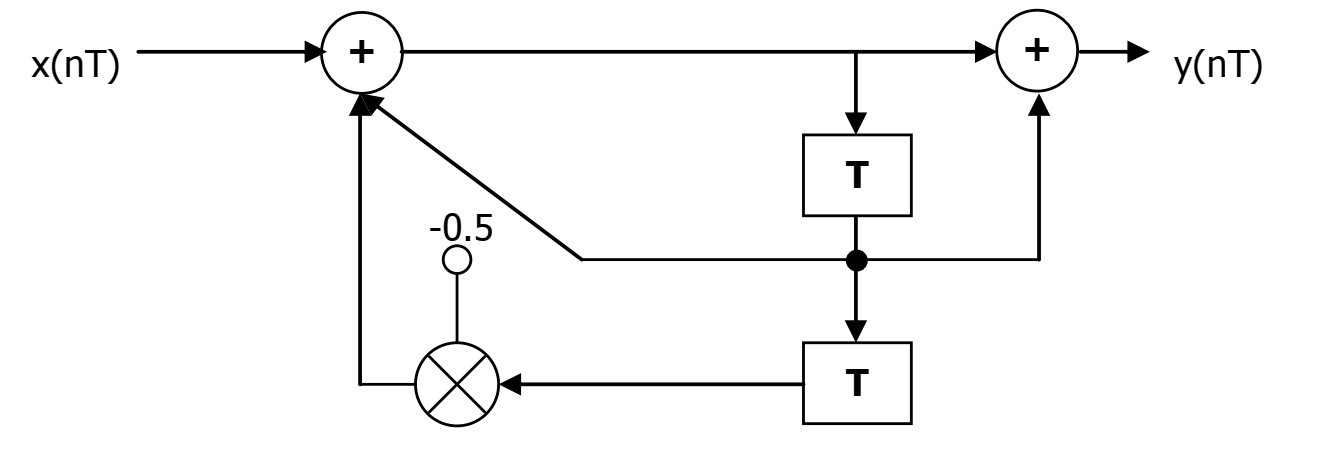
\includegraphics[width = .5\textwidth]{Red.png}
    \label{fig:Red}
\end{figure}
Creando una variable intermedia e(nT), tenemos que el esquema de la red cambia a:
\begin{figure}[H]
    \centering
    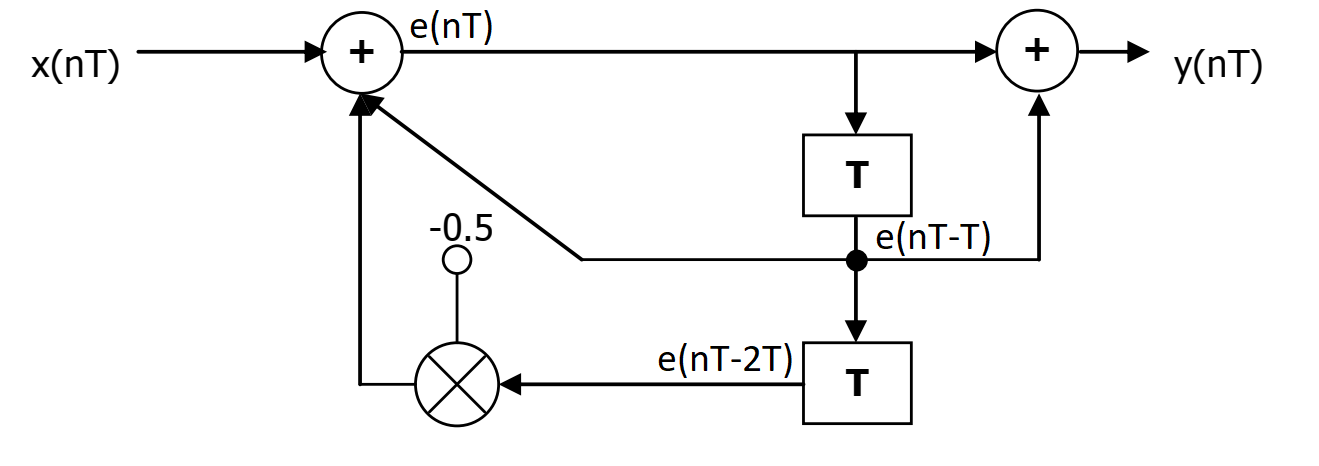
\includegraphics[width = .5\textwidth]{RedEstudiada.png}
    \label{fig:Red}
\end{figure}
Obtenemos las siguientes ecuaciones:\\
\begin{equation*}
\left\{
\begin{aligned}
y(nT) & = e(nT) + e(nT-T) \\
e(nT) & = x(nT) + e(nT-T) -0,5 e(nT-2T)
\end{aligned}
\right.
\end{equation*}

A partir de la ecuaci\'on de y(nT), obtengo que $e(nT-T)=y(nT)-e(nT)$ y reemplazando esto en la otra ecuaci\'on terminamos obteniendo:
$$e(nT)= x(nT) + e(nT-T) -0,5 [y(nT-T)-e(nT-T)]$$
$$e(nT)= x(nT) + 1,5e(nT-T) -0,5y(nT-T)$$
$$e(nT)= x(nT) + 1,5[y(nT)-e(nT)] -0,5y(nT-T)$$
$$2,5e(nT)= x(nT) + 1,5y(nT) -0,5y(nT-T)$$
$$e(nT)= \frac{2}{5} x(nT) + \frac{3}{5}y(nT) -\frac{1}{5}y(nT-T)$$
Utilizando la formula reci\'en obtenida para e(nT) en la ecuaci\'on de y(nT), conseguimos:
$$y(nT) = \left[ \frac{2}{5} x(nT) + \frac{3}{5}y(nT) -\frac{1}{5} y(nT-T)\right] + \left[ \frac{2}{5} x(nT-T) + \frac{3}{5} y(nT-T) -\frac{1}{5} y(nT-2T)\right]$$
$$y(nT) =  \frac{2}{5} x(nT)  + \frac{2}{5} x(nT-T) + \frac{3}{5}y(nT) + \frac{2}{5} y(nT-T) -\frac{1}{5} y(nT-2T)$$
$$\frac{2}{5}y(nT) =  \frac{2}{5} x(nT)  + \frac{2}{5} x(nT-T) + \frac{2}{5} y(nT-T) -\frac{1}{5} y(nT-2T)$$
Finalmente obteniendo la siguiente ecuación diferencial:
$$y(nT) =  x(nT)  + x(nT-T) + y(nT-T) -0,5 y(nT-2T)$$
\end{document}